%CS 109 Problem Set Xiaoqi Zhou


\documentclass{article}
	% basic article document class
	% use percent signs to make comments to yourself -- they will not show up.

\usepackage{amsmath}
\usepackage{amssymb}
	% packages that allow mathematical formatting

\usepackage{graphicx}
\usepackage{float}
	% package that allows you to include graphics

\usepackage[top=1in, bottom=1in, left=1in, right=1in]{geometry}

\frenchspacing
	% one space after periods

\usepackage{fancyhdr}
	% allows custom headers

\pagestyle{fancy}

\lhead{CS 109, Stanford University \\ Problem Set \#2} 
\rhead{Xiaoqi Zhou (xqzhou@stanford.edu) \\ 06237147}
\usepackage{color}
\usepackage{courier}
\cfoot{\thepage}
\renewcommand{\footrulewidth}{0.4pt} 
	%footer
\newcommand{\myansw}{\textbf{Answer:}\\}
\newcommand{\mysolu}{\textbf{Solution:}\\}
\begin{document}
\thispagestyle{fancy} %shows header/footer

\begin{enumerate}
	\item
	\begin{enumerate}
		%1.a
		\item
		\mysolu
		Define event\\
		${J = \{\text{engineer program in Java}\}}$\\
		${C = \{\text{engineer program in C++}\}}$\\
		Then
		${P(C|J)=\frac{P(CJ)}{P(J)}}$\\
		${0.24=\frac{P(CJ)}{0.36}}$\\
		\myansw
		The probability that a randomly selected engineer programs in Java and C++ is\\
		\colorbox{yellow}{
			${P(CJ)=0.0864}$\\
		}\\
		%1.b
		\item
		\mysolu
		${P(J|C)=\frac{P(CJ)}{P(C)}}$\\
		\myansw
		The probability that a randomly selected engineer programs in Java given that he/she programs in C++ is\\
		\colorbox{yellow}{
			${P(J|C)=\frac{0.0864}{0.33}=0.2618}$\\
		}\\
	\end{enumerate}
	\item
	\begin{enumerate}
		%2.a
		\item 
		\mysolu
		${P(E)=\frac{4\times 3}{52 \times 51}=0.00452}$\\
		The Ace of Spades can be either the first card or the second card\\
		${P(F)=\frac{1\times 51 + 51 \times 1}{52 \times 51}=0.0385}$\\
		${P(EF)=\frac{1\times 3 + 3 \times 1}{52 \times 51}=0.00226}$\\
		\myansw
		\colorbox{yellow}{${P(E|F)=\frac{P(EF)}{P(F)}=0.0588}$}\\
		%2.b
		\item 
		\mysolu
		Since event ${G}$ must happen when event ${E}$ happens\\
		${P(G|E)=1}$\\
		${1=\frac{P(GE)}{P(E)}}$\\
		${P(GE)=P(E)}$\\
		We can calculate the complement of event ${G}$\\
		${P(G^c)=\frac{48\times 47}{52\times 51}=0.851}$\\
		${P(G)=1-P(G^c)=0.149}$\\
		\myansw
		\colorbox{yellow}{
			${P(E|G)=\frac{P(EG)}{P(G)}=\frac{P(E)}{P(G)}=0.0303}$
		}\\
	\end{enumerate}
	\item
	\begin{enumerate}
		\item
		\mysolu
		Define event ${E_i=\{\text{a user likes movie} M_i\}}$,${T=\{\text{a user like the Tearjerker genre}\}}$\\
		${P(E_i|T)=p_i}$\\
		\myansw
		${P((E_1 \cap E_2 \cap E_3)|T)=P(E_1|T)\cap P(E_2|T)\cap P(E_3|T)}$\\
		Since all the ${E_i|T}$ are conditionally independent, the probability that a user likes all three movies $M_1$, $M_2$ and $M_3$ given that they like the Tearjerker genre is\\
		${P((E_1 \cap E_2 \cap E_3)|T)=P(E_1|T)P(E_2|T)P(E_3|T)=p_1 p_2 p_3}$
		\item
		\myansw
		\colorbox{yellow}{
			${P((E_1 \cup E_2 \cup E_3)|T)=P(E_1|T) \cup P(E_2|T) \cup P(E_3|T) = p_1+p_2+p_3 - (p_1 p_2+p_3 p_2+p_3 p_1)+p_1p_2p_3}$
		}\\
		\item
		\mysolu
		Define event ${E_{all}=\{\text{user likes all the 3 movie}\}}$\\
		${P(E_{all}|T)=p_1 p_1 p_3}$\\
		${P(E_{all}|T^c)=q_1 q_2 q_3}$\\
		${P(E_{all}T)=P(E_{all}|T)P(T)=0.6 p_1 p_2 p_3}$\\
		${P(E_{all}T^c)=P(E_{all}|T^c)P(T)=(1-0.6) q_1 q_2 q_3=0.4 q_1 q_2 q_3 }$\\
		${P(E_{all})=P(E_{all}T)+P(E_{all}T^c)}$\\
		\myansw
		The probability that they like the Tearjerker genre that they like $M_1$, $M_2$ and $M_3$ is\\
		\colorbox{yellow}{
			${P(T|E_{all})=\frac{P(TE_{all})}{P(E)}=\frac{0.6 p_1 p_2 p_3}{0.6 p_1 p_2 p_3+0.4 q_1 q_2 q_3}}$
		}\\
		
	\end{enumerate}
	\item
	\begin{enumerate}
		\item
		\mysolu
		We can calculate the probability of event ${F=\{text{all the 5 servers failed in one year}\}}$\\
		${P(F)=(1-p)^5}$\\
		\myansw
		The probability that at least 1 server is still working after on year is\\
		\colorbox{yellow}{${P(E_1)=1-P(F)=1-(1-p)^5}$}\\
		\item
		\mysolu
		We can consider each particular combination of the 3 servers that are still working.\\
		${P(G_i)=p^3(1-p)^2}$\\
		Since all the events are mutually exclusive
		\myansw
		The probability that exactly 3 server is still working after on year is\\
		\colorbox{yellow}{
			${P(E_3)={5 \choose 3}P(G_i)=10p^3(1-p)^2}$
		}\\
		\item
		\mysolu
		We can consider 3 situations: exactly 3, 4, 5 servers are still working after one year and combine them together.\\
		\myansw
		The probability that at least 3 server is still working after on year is\\
		\colorbox{yellow}{
			${P(E)=P(E_3)+P(E_4)+P(E_5)=\sum\limits_{i=3}^5 {5 \choose i}p^i(1-p)^{5-i}}$
		}\\
		
	\end{enumerate}
	\item
	\mysolu
	The probability of all the bit is 0 in a ${n}$ bit string is\\
	${P(F) = (1-p)^n}$\\
	Then the probability that at least one 1 in the string is\\
	${P(E) = 1- P(F)= 1-(1-p)^n}$\\
	\myansw
	${P(E)>0.7}$\\
	The ${n}$ requirment for the probability that there is at least one 1 in the string is at least 0.7 is\\
	\colorbox{yellow}{	
		${n>log_{1-p}(0.3)}$
	}\\
	\item
	\begin{enumerate}
		\item
		\mysolu
		${F_i=\{\text{at least one string hashed into i-th bucket}\}}$\\
		${P(E) = 1-P((F_1 F_2 F_3 F_4)^c)=1-P(F_1^c \cup F_2^c \cup F_3^c \cup F_4^c)}$\\
		Since all the ${F_i^c}$ are not mutually exclusive, the answer will be very complex before expansion.
		Because of the limited number of buckets and strings, we can try to use another way to get the answer.\\
		${G = \{\text{All the buckets have at least 1 string}\}}$\\
		${H = \{\text{No string in bucket 5, all the first 4 buckets have  one or 2 strings}\}}$\\
		${I = \{\text{No string in bucket 5, all the first 4 buckets have  one or 3 strings}\}}$\\
		${P(E)=P(G)+P(H)+P(I)}$\\
		For each of event ${G}$, there is only one bucket can have 2 strings in it and we can add up all the 5 possible situation to get the total probability.\\
		${P(G)=\frac{6!}{2!}\sum\limits_{i=1}^5(p_i\prod\limits_{j=1}^5p_j)=360\sum\limits_{i=1}^5 p_i\prod\limits_{j=1}^5p_j = 360\prod\limits_{j=1}^5p_j}$\\
		For each of event ${H}$, there are 2 bucket have 2 strings in it.\\
		${P(H)=\frac{6!}{2!2!}(p_1 p_2 p_3^2 p_4^2+p_1 p_2^2 p_3 p_4^2 \ldots)=180(p_1 p_2 + p_1 p_3 + p_1 p_4 + p_2 p_3 + p_2 p_4 + p_3 p_4)p_1 p_2 p_3 p_4}$\\
		For each of event ${H}$, there are 1 bucket have 3 strings in it.\\
		${P(I)=\frac{6!}{3!}(p_1^3 p_2 p_3 p_4 + p_1 p_2^3 p_3 p_4 + p_1 p_2 p_3^3 p_4+ p_1 p_2 p_3 p_4^3) = 120(p_1^2+p_2^2+p_3^2+p_4^2) p_1 p_2 p_3 p_4}$\\
		\myansw
		\colorbox{yellow}{
		${P(E)=60(6p_5 + 3(p_1 p_2 + p_1 p_3 + p_1 p_4 + p_2 p_3 + p_2 p_4 + p_3 p_4)+2(p_1^2+p_2^2+p_3^2+p_4^2))p_1p_2p_3p_4}$}\\
		\item
		\myansw
		After substitute all the ${p_i}$ values, we can get\\
		\colorbox{yellow}{
			${P(E)=60\times(6\times 0.1 + 3\times 0.2925+2\times 0.225)\times 0.001875=0.2168}$
		}
		
	\end{enumerate}
	\item
	\begin{enumerate}
		\item
		\mysolu
		The probability that \textbf{\texttt{fairRandom}} returns 1 can be described as\\
		${P({r2 = 1|r2\neq r1})=\frac{P(\{r2 = 1, r1 = 0\})}{P(\{r2 \neq r1\})}}$\\
		\myansw
		The probability that \textbf{\texttt{fairRandom}} returns 1 is\\
		\colorbox{yellow}{${P(E)= \frac{p(1-p)}{p(1-p)+(1-p)p}=0.5}$}\\
		So that \textbf{\texttt{fairRandom}} dose indeed return a 0 and a 1 with equal probability.
		\item
		\mysolu
		Based on the \textbf{\texttt{simpleRandom}}, the only chance that function can return is when ${r2 \neq r1}$. So we can find\\
		${P(\{r2 = 1|r1 = 1\})=0}$\\
		${P(\{r2 = 1|r1 = 0\})=1}$\\
		The probability of ${P(\texttt{simpleRandom}\text{ returns 1})}$ is\\
		\colorbox{yellow}{
		${P(\{r2 = 1\})=P(\{r1=0\})=1-p}$}\\
		\myansw
		We can not guarantee that \textbf{\texttt{simpleRandom}} generates 0's and 1's with equal probability unless \textbf{\texttt{unknownRandom}} returns 0's and 1's with equal probability ${p = 0.5}$.
		\item
		\mysolu
		After run the simulation, the probability that second player wins is\\
		\colorbox{yellow}{${P(\{\text{second player wins}\}) = 0.516}$}\\
		Assuming all the random numbers are integers.\\
		If the random number can be decimals, the simulation result is\\
		\colorbox{yellow}{${P(\{\text{second player wins}\}) = 0.528}$}\\
		The difference between simulation results of simulation in integers and decimals is because of the probability that first and second player have the same number is more obvious when we use integers in simulation.
		The condition when first and second player start the game is not equivalent. The first player always starts at ${S=0}$. The rule to the second player is equivalent to that stop when ${S>100}$ but the start point is ${S = X}$, ${X}$ is the residual of the first player.
		Since second player's turn ends by the larger numbers in the first trial is higher than the first player, the chance of the second player has larger last number is higher than first player.
	 		
	\end{enumerate}
	\item
	\mysolu
	We can define the event ${E=\{\text{window is detected}\}}$. Then\\
	${P(EL_1)=0.8\times 0.2=0.16}$\\
	${P(EL_2)=0.2\times 0.9=0.18}$\\
	Since ${L_1}$ and ${L_2}$ are complement to each other,\\
	${P(E)=P(EL_1)+P(EL_2)=0.34}$\\
	We can update the probability estimation based on the new information that the window is detected.
	${P(L_1|E)=\frac{P(EL_1)}{P(E)}=0.47}$\\
	${P(L_2|E)=\frac{P(EL_2)}{P(E)}=0.53}$\\
	\myansw
	The robot new values for ${P(L_1)}$ and ${P(L_2)}$ is\\
	\colorbox{yellow}{
		${P(L_1')=P(L_1|E)=0.47}$
	}\\
	\colorbox{yellow}{
		${P(L_2')=P(L_2|E)=0.53}$
	}\\

	\item
	\mysolu
	For each location we can define the probability of the cell at that location is ${P(L_i)}$; the probability of a cell records two bars is ${P(B)}$\\
	${P(B|L_i)=\frac{P(BL_i)}{P(L_i)}}$\\
	${P(BL_i)=P(L_i)P(B|L_i)}$\\
	Since the summation of the probability that records two bars at all the locations is the total probability that the cell can have two bars.\\
	${P(Li|B)=\frac{P(BL_i)}{P(B)}=\frac{P(L_i)P(B|L_i)}{\sum\limits_{i=1}^n P(L_i)P(B|L_i)}}$\\
	In the program, we can calculate ${P(BL_i)}$ in each location and get the summation of them.\\
	\myansw
	The probabilities of all 16 cells is\\
	\colorbox{yellow}{
		$\begin{bmatrix}
			0.0744&0.1885&0.0744&0.0050\\
			0.0050&0.1488&0.0942&0.0744\\
			0.0010&0.0050&0.1488&0.0942\\
			0.0010&0.0010&0.0010&0.0744\\
		\end{bmatrix}$
	}
	\item
	\begin{enumerate}
		\item
		\mysolu
		Assume A is the blue-eyed genes and B is the brown-eyed gene. Since William's sister have blue eye and William and both of his parents have brown eyes, we can know that both of William's parents are (AB) combination.
		The possible gene combinations of William is (AA), (AB), (BA), (BB). Define ${E = \{\text{William possesses a blue-eyed gene}\}}$, ${F = \{\text{William has brown eyes}\}}$.\\
		${P(F) = \frac{3}{4}}$\\
		${P(E)= \frac{2}{4} = \frac{1}{2}}$\\
		\myansw
		The probability that William possesses a blue-eyed gene is\\
		\colorbox{yellow}{${P(G)=P(E|F)=\frac{P(EF)}{P(F)}=\frac{0.5}{0.75}=\frac{2}{3}}$}\\
		\item
		\mysolu
		William's wife have blue eyes, that means her gene combination is (AA).\\
		Define ${H = \{\text{William's first child have blue eyes}\}}$\\
		${P(H) = P(HG)+P(HG^c)={P(H|G)}{P(G)}+{P(H|G^c)}{P(G^c)}}$\\
		\myansw
		The probability that their first child will have blue eyes is\\
		\colorbox{yellow}{${P(H) = \frac{1}{2} \times \frac{2}{3}+\frac{1}{3} \times 0 = \frac{1}{3}}$}\\
		\item
		\mysolu
		Define ${I = \{\text{William's next child have brown eyes}\}}$, so ${I^c = \{\text{William's next child have blue eyes}\}}$\\
		We should update event ${G = \{\text{William possesses a blue-eyed gen}\}}$, based on knowing that his first child have brown eyes.\\
		${P(G')=P(G|H^c)=\frac{P(GH^c)}{P(H^c)}=\frac{\frac{1}{3}}{\frac{2}{3}}=\frac{1}{2}}$\\
		\myansw
		By using the previous conclusion\\
		${P(I^c)= P(I^c|G')P(G)+P(I^c|G'^c)P(G'^c)=\frac{1}{2}\times \frac{1}{2}+0 \times \frac{1}{3} = \frac{1}{4}}$\\
		The probability that their next child will also have brown eyes is\\
		\colorbox{yellow}{${P(I)=1-P(I^c) = \frac{3}{4}}$} \\
		
	\end{enumerate}
	\item
	\begin{enumerate}
		\item
		\mysolu
		From the description, we can find\\
		${P(T_1|G^c) = 0}$\\
		${P(T_2|G^c) = 0}$\\
		${P(T_1 T_2|G^c) = 0.72}$\\
		\myansw
		${P(T_1|G)P(T_2|G)=P(T_1 T_2|G)=0.72}$\\
		\colorbox{yellow}{So, ${T_1}$ and ${T_2}$ are conditionally independent given ${G}$.}\\
		\item
		\myansw
		${P(T_1|G)=P(T_2|G) = 0}$\\
		\colorbox{yellow}{Since both of the probability is 0, ${T_1}$ and ${T_2}$ conditionally independence is undifined ginve ${G^c}$}\\
		\item
		\myansw
		\colorbox{yellow}{${P(T_1)= P(T_1|G)P(G)+P(T_1|G^c)P(G^c) = 0.8\times 0.6 = 0.48}$}\\
		\item
		\myansw
		\colorbox{yellow}{${P(T_2)= P(T_2|G)P(G)+P(T_2|G^c)P(G^c) = 0.9\times 0.6 = 0.54}$}\\
		\myansw
		${P(T_1 T_2)= P(T_1 T_2|G)P(G)=0.72\times 0.6 = 0.432}$\\
		${P(T_1)P(T_2)=0.48\times 0.52 = 0.2592}$\\
		${P(T_1)P(T_2) \neq P(T_1 T_2)}$\\
		\colorbox{yellow}{${T_1}$ and ${T_2}$ are NOT independent (gene G is the relation ship between them.)}\\
	\end{enumerate}
	\item
	\begin{enumerate}
		\item
		\myansw
		\colorbox{yellow}{${P(T) = 0.30079}$}\\
		\item
		\myansw
		\colorbox{yellow}{${P(G_1) = 0.70028}$}\\
		\colorbox{yellow}{${P(G_2) = 0.30076}$}\\
		\colorbox{yellow}{${P(G_3) = 0.5009}$}\\
		\colorbox{yellow}{${P(G_4) = 0.8016}$}\\
		\colorbox{yellow}{${P(G_5) = 0.32705}$}\\
		\item
		\mysolu
		${P(G_1T) = 0.21210 }$ vs. ${P(G1)P(T) = 0.21124}$\\
		${P(G_2T) = 0.09089}$ vs. ${P(G2)P(T) = 0.09047}$\\
		${P(G_3T) = 0.29212}$ vs. ${P(G3)P(T) = 0.15067}$\\
		${P(G_4T) = 0.29703}$ vs. ${P(G4)P(T) = 0.24112}$\\
		${P(G_5T) = 0.29434}$ vs. ${P(G5)P(T) = 0.09837}$\\
		\myansw
		\colorbox{yellow}{${G_1}$ and ${G_2}$ independent of ${T}$, ${G_4}$ is likely independent of ${T}$}\\
		
		\item
		\myansw
		${P(T|G_1)=\frac{P(G_1T)}{P(G_3)} = 0.302}$ independent\\
		${P(T|G_2)=\frac{P(G_2T)}{P(G_3)} = 0.302}$ independent\\
		\colorbox{yellow}{${P(T|G_3)=\frac{P(G_3T)}{P(G_3)} = 0.583}$} double the chance to have trait\\
		${P(T|G_4)=\frac{P(G_4T)}{P(G_4)} = 0.371}$  likely independent\\
		\colorbox{yellow}{${P(T|G_5)=\frac{P(G_5T)}{P(G_5)} = 0.900}$} important fact to have trait\\
		
		\item
		\myansw
		For the previous results we can find\\
		\colorbox{yellow}{1. ${G_5}$ is assumed to be a main course of the trait}\\
		\colorbox{yellow}{2. ${G_3}$ is assumed to increase the probability of the trait}\\
		\colorbox{yellow}{3. ${G_4}$ is assumed to have some relationship between the trait}\\
		
		\item
		\mysolu
		We can always create a program to ergodic the relationships between all the combination of genes and automatically figure out the independences. Based on the limited size of gene that we are interested in, we can have a other way to find the hidden rule to guide our analysis.\\
		We create a pattern number based on the combination of gene. For all the 6 gene, we can have pattern 0 to 31, and each pattern can represent one of the distinct gene combination. For example, combination ${G_5 G_4^c G_3 G_2 G_1^c}$ and be represented as b10110 = 22.\\
		Following is the plot of counts of samples in different gene pattern.\\
		\begin{figure}[H]
			\caption{Trait vs. Gene Pattern}
			\centering
			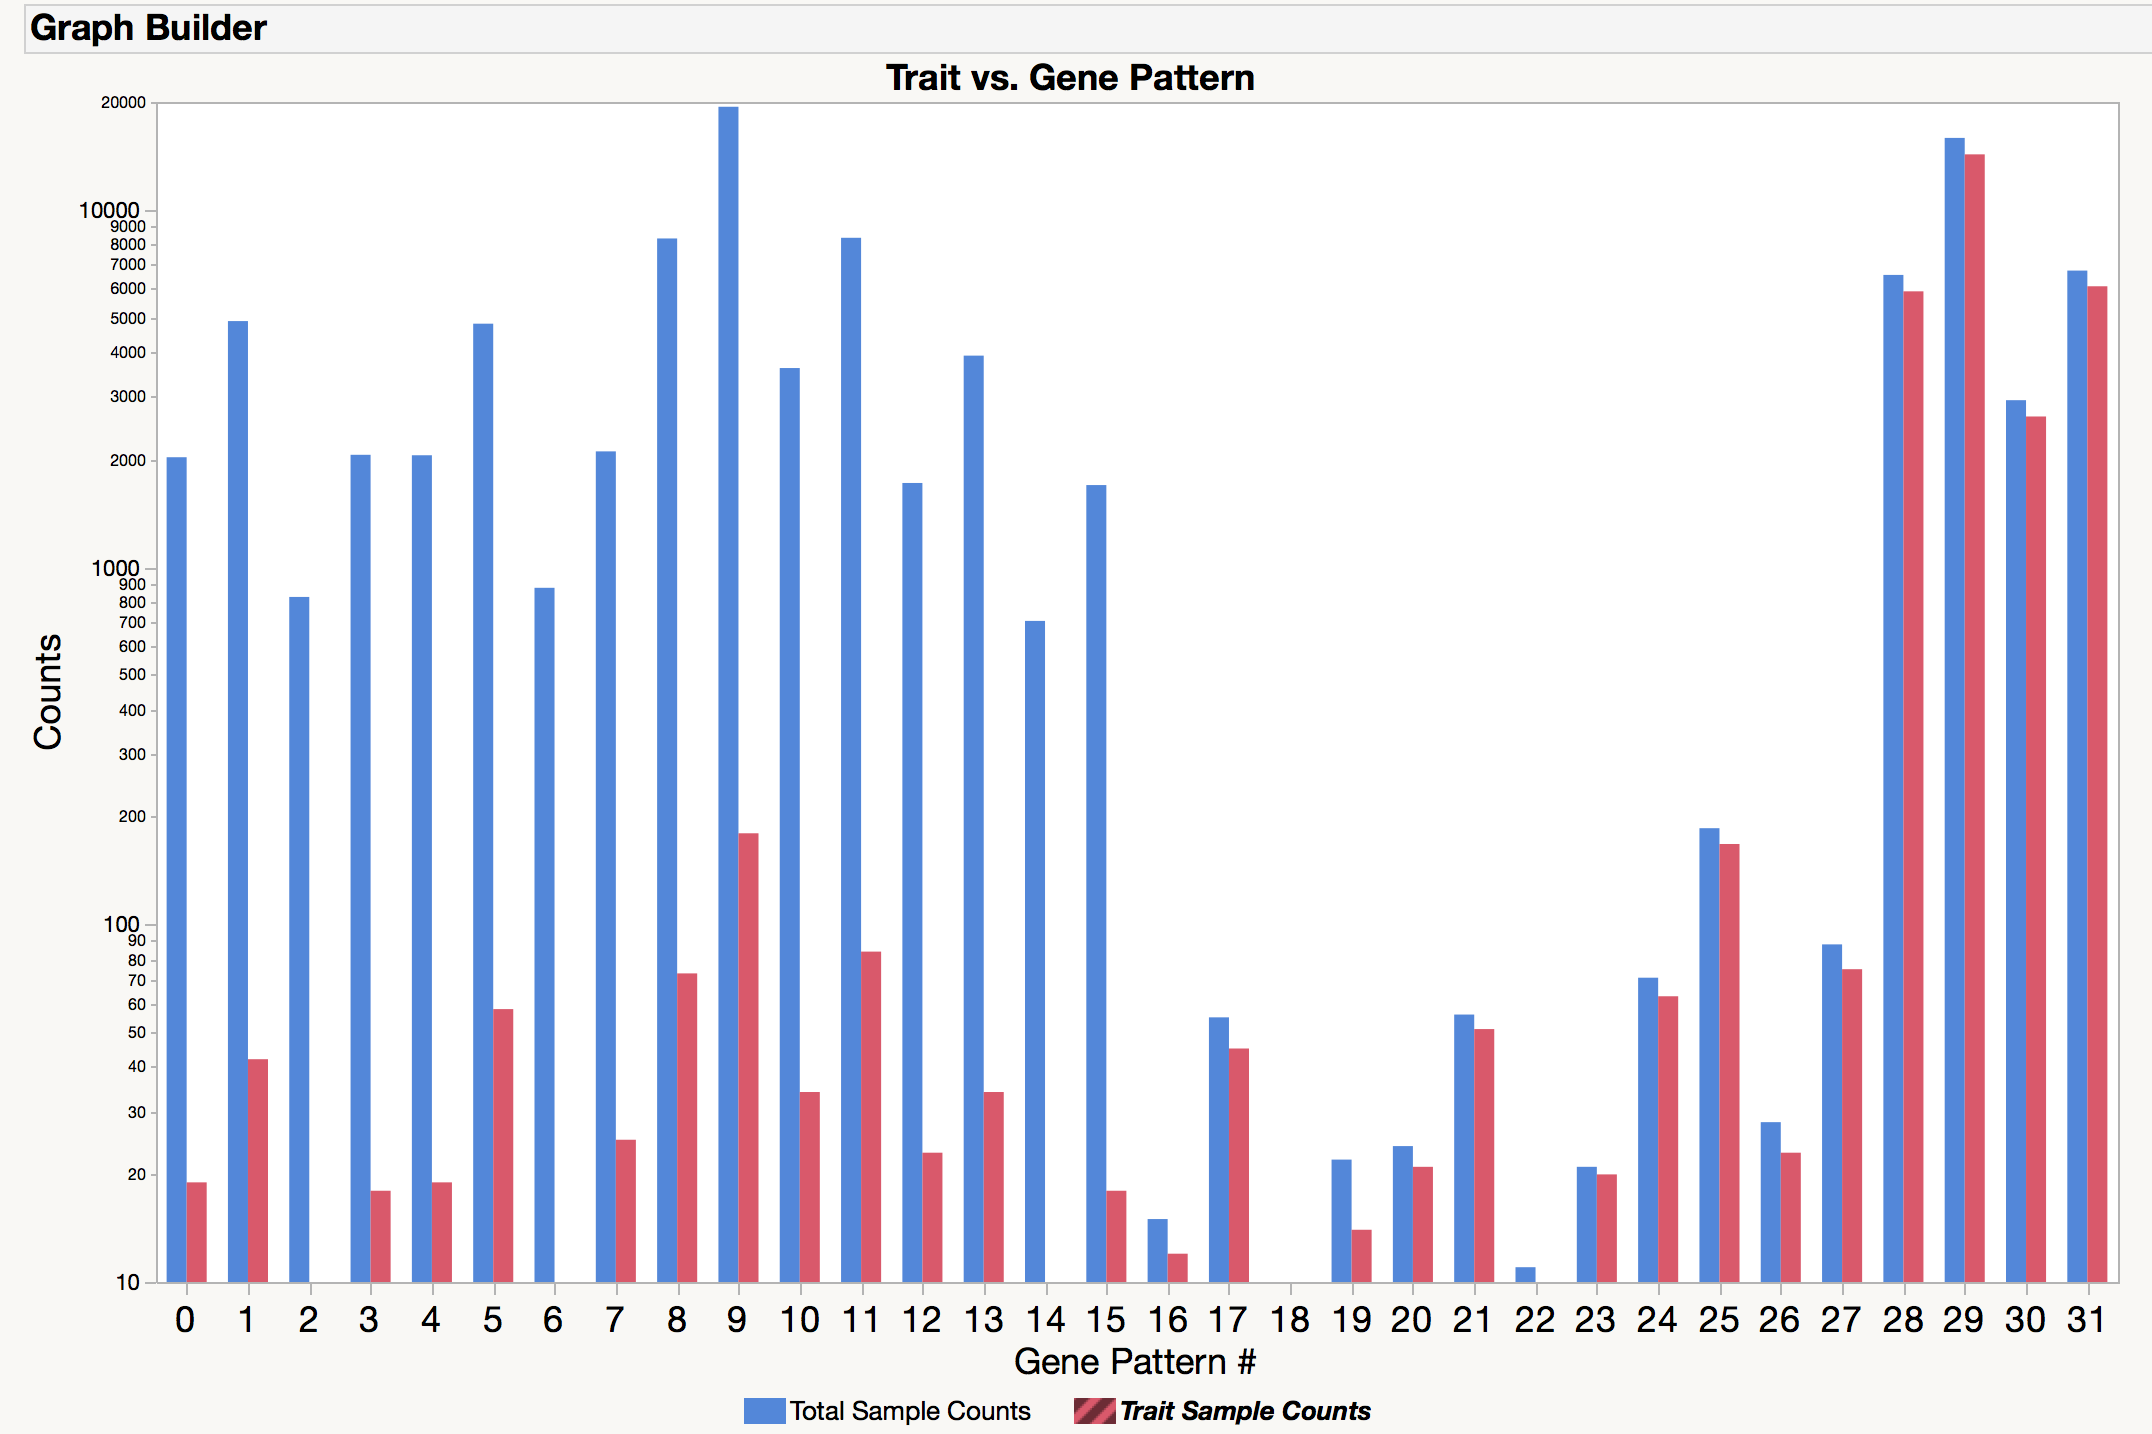
\includegraphics[width=0.8\textwidth]{bat.png}
		\end{figure}
		Becasue of the high dynamic range of the sample counts in different gene pattern, the Y scale of the plot is set to log. We can find that ${G_5}$ only exist when both ${G_3}$ and ${G_4}$ exist.\\
		${P(G_5|G_3G_4)=0.800}$\\
		${P(G_3G_4|G_5) =0.982}$\\
		\colorbox{yellow}{${G_3 \cap G_4}$ is the necessity condition of ${G_5}$}\\
		${P(G_3G_4) = 0.401}$ vs.${P(G_4)P(G_4)=0.402}$\\ 
		\colorbox{yellow}{${G_3}$ and ${G_4}$ are independent.}\\
		Given ${P(T|G_5) = 0.900}$, not all the bats with ${T}$ have ${G_5}$. If we still believe ${G_5}$ is necessity condition of ${T}$, we can analysis the fales positive rate of the experiment or test for trait.\\
		If ${P\{\text{false positive}\} > P{(T|G_5^c)}=0.049}$, it is very likely the trait without ${G_5}$ is casued by fales positive in the test.\\
		Same as the samples have ${G_5}$ but not trait.\\
		If ${P\{\text{false negative}\}>P(G_5|T)=0.020}$, it is very likely that the sample have ${G_5}$ but not have ${T}$ is casued by false negative in the test.\\
				\begin{figure}[H]
			\caption{Gene and Trait Relationship}
			\centering
			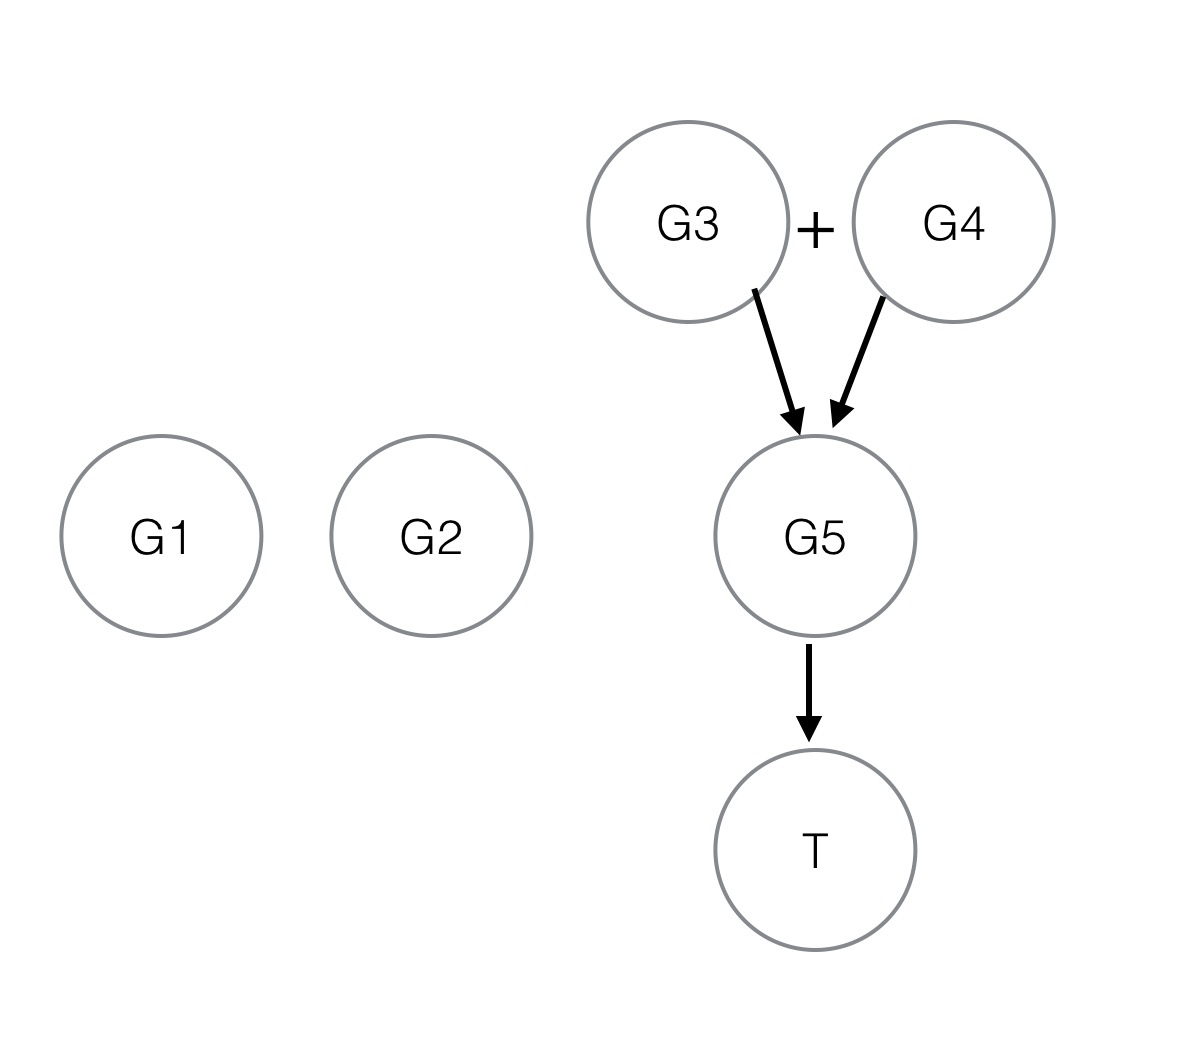
\includegraphics[width=0.5\textwidth]{GT.jpg}
		\end{figure}
		
		

	\end{enumerate}


%	\item A product in math mode: \[\prod\limits_{i=1}^n x = x^n\]



\end{enumerate}

\newpage


\end{document}